\documentclass[a4paper, 12pt]{report}

\usepackage[italian]{babel}
\usepackage{graphicx}
\usepackage{float}
\usepackage{tabularx}
\usepackage{ltablex}
\usepackage[font=small,format=plain,labelfont=bf,up,textfont=normal,up,justification=justified,singlelinecheck=false,skip=0.01\linewidth]{caption}
\usepackage{tikz}
\renewcommand{\familydefault}{\sfdefault}

\title{Assignment 3 - Programmazione di reti\newline Anno accademico 2018-2019}
\date{\today}

\author{Matteo Castellucci - 0000825436\\Elena Rughi - 0000832797\\Yuqi Sun - 0000826197\newline}

\begin{document}

\maketitle
\tableofcontents

\chapter{Task Uno}

\begin{figure}[H]
	\centering
	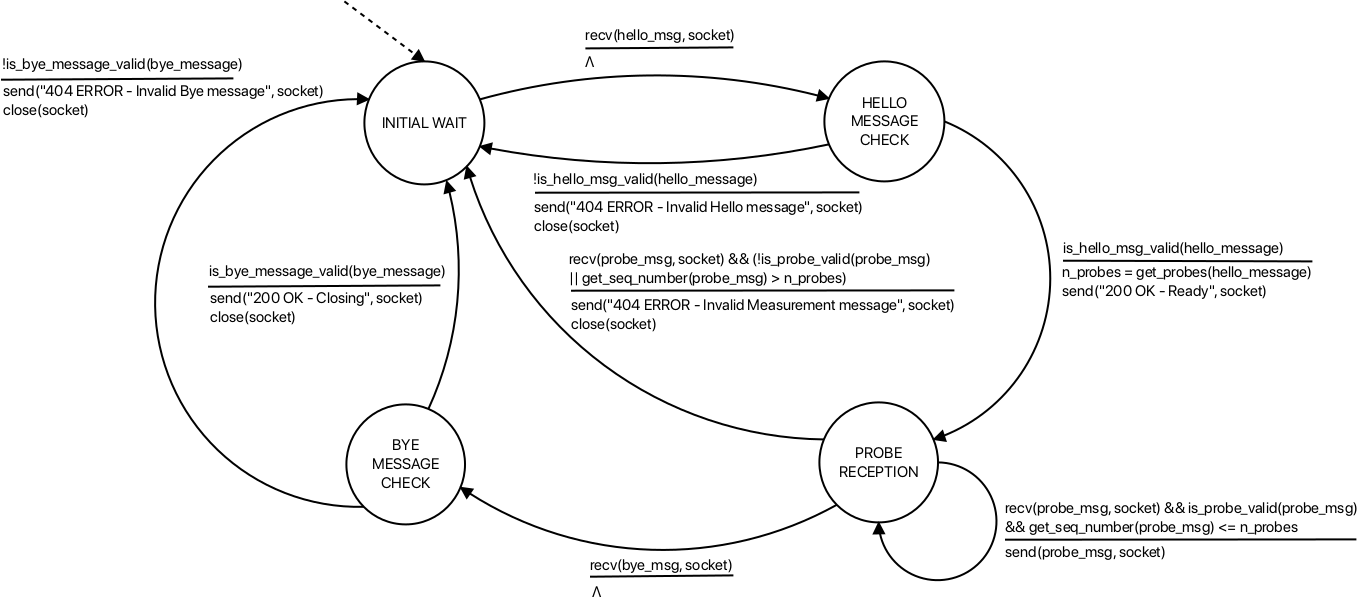
\includegraphics[width=\linewidth]{images/fsm_server.png}
	\caption{\textit{Finite State Machine} che rappresenta il comportamento del \textit{server}}
\end{figure}

\begin{figure}[H]
	\centering
	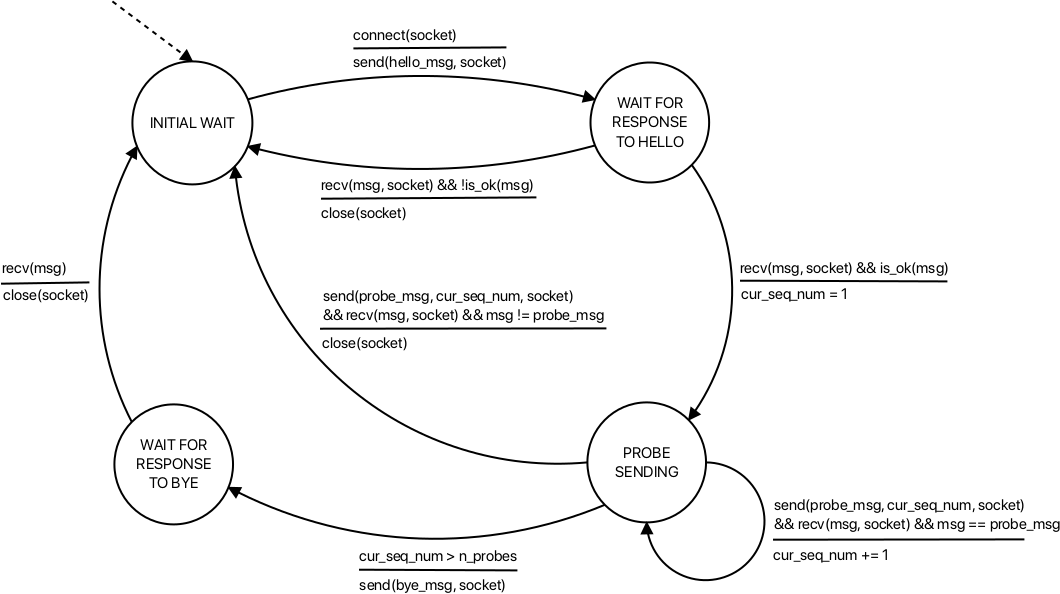
\includegraphics[width=\linewidth]{images/fsm_client.png}
	\caption{\textit{Finite State Machine} che rappresenta il comportamento del \textit{client}}
\end{figure}

Sia il \textit{client} che il \textit{server} partono da uno stato di attesa iniziale, denominato ``\textit{initial wait}". Il \textit{server}
rimane in attesa di nuovi \textit{client} che hanno intenzione di connettersi e inviare un ``\textit{hello message}" per iniziare la comunicazione,
mentre il \textit{client} rimane in attesa di potersi connettere con il \textit{server} e poter inviare l'``\textit{hello message}".\newline
Una volta che il \textit{server} riceve l'``\textit{hello message}", esso entra nella cosiddetta ``\textit{hello phase}", il
\textit{client} vi entra nel momento in cui riesce ad inviare l'``\textit{hello message}".

\section{Hello phase}

Alla ricezione dell'``hello message" inviato dal \textit{client}, il server entra nello stato di ``\textit{hello message check}", dove esso
si preoccupa di controllare che esso sia valido secondo le specifiche del protocollo. Se il messaggio non è valido, il server notifica il
\textit{client} con un messaggio di errore e chiude la connessione, ritornando allo stato iniziale. In caso contrario, il \textit{server}
invia un messaggio di conferma e passa alla ``\textit{measurement phase}".\newline
Il \textit{client}, ora nello stato di ``\textit{wait for response to hello}", attende una risposta all'``hello message" inviato. Se riceve
un messaggio di errore come risposta termina anche lui la connessione e ritorna allo stato iniziale, altrimenti anche lui entra nella
``\textit{measurement phase}".

\section{Measurement phase}

Trovandosi nello stato di ``\textit{probe sending}", il \textit{client} si preoccupa di inviare i ``\textit{probe message}" correttamente ed in 
sequenza.\newline
Il server si trova invece nello stato di ``\textit{probe reception}". Perciò, al ricevimento di un ``\textit{probe message}", il \textit{server}
controlla che esso abbia il numero di sequenza corretto, utilizzando un proprio contatore interno, che sia valido secondo le specifiche del protocollo
e non ecceda il numero di ``\textit{probe message}" che il \textit{client} aveva intenzione di inviare, valore estratto dall'``\textit{hello message}" inviato in precedenza.\newline
In caso il ``\textit{probe message}" non sia valido secondo i controlli indicati poc'anzi, il \textit{server} invia un messaggio di errore e chiude
la connessione, ritornando allo stato iniziale. Altrimenti, invia il ``\textit{probe message}" ricevuto al \textit{client}.\newline
Il \textit{client}, in caso ricevesse indietro il ``\textit{probe message}" appena inviato al \textit{server} significa che l'invio è andato a buon fine
e può proseguire, altrimenti chiude la connessione e ritorna allo stato iniziale.\newline
Questa fase termina con successo nel momento in cui il \textit{client} ha inviato il numero di ``\textit{probe message}" che aveva specificato 
nell'``\textit{hello message}", a cui fa seguire l'invio del ``\textit{bye message}", entrando nella ``\textit{bye phase}".\newline
Alla ricezione del ``\textit{bye message}", anche il server entra nella ``\textit{bye phase}".

\section{Bye phase}

Il \textit{server}, ora nello stato di ``\textit{bye message check}" controlla che tale messaggio inviatogli dal \textit{client} sia corretto
secondo le specifiche del protocollo.\newline
Il server risponde al ``\textit{bye message}" con un messaggio di errore nel caso non fosse valido, di conferma in caso contrario.
In entrambi i casi, il \textit{server} chiude la connessione e ritorna allo stato di attesa iniziale.\newline
Il \textit{client}, nello stato di ``\textit{wait for response to bye}", attende la ricezione del messaggio di risposta al ``\textit{bye message}"
inviato e, una volta ricevuto, chiude la connessione, ritornando allo stato di attesa iniziale.

\chapter{Task Due}

\section{Strategia risolutiva adottata per l'implementazione di client e server}

\subsection{Server}

Il server per essere eseguito necessita di ricevere la porta della \textit{socket} su cui si metterà in ascolto per nuove connessioni in ingresso
come parametro iniziale.\newline
Dopo aver creato la \textit{socket} TCP di benvenuto, il \textit{server} entra in un \textit{loop} infinito dove si mette in ascolto per eventuali
richieste di connessione da parte dei \textit{client}; in questo modo, dopo la chiusura di una connessione, il \textit{server} torna in ascolto,
eliminando così la necessità di riavviare il programma.\newline
Dopo avere registrato l'indirizzo IP e la porta del \textit{client}, il server si mette in attesa dell'``\textit{hello message}". Una volta
ricevuto ed assicuratosi che sia valido, salva i dati in esso contenuti in un'apposita \textit{struct} di tipo ``struct hello\_msg". In seguito,
tramite un ciclo ``for", si mette in attesa di un numero ``probe message" pari a quello estratto dall'``\textit{hello message}". La ricezione di
un ``probe message" avviene in un ciclo ``do-while" perché in alcuni test è risultato che la funzione ``recv" non riuscisse a leggere più di
32.768 byte alla volta, mentre alcuni di questi messaggi risultavano più lunghi di questa quantità. In questo modo, leggendo il messaggio 
un po' alla volta, si riesce ad ottenerlo tutto. Dopo aver controllato che
il messaggio sia valido, il \textit{server} attende il numero di secondi specificato come ``\textit{server delay}" nell'``\textit{hello message}"
prima di inviare lo stesso messaggio indietro al \textit{client}.\newline
Finiti i ``\textit{probe message}", il server si mette in attesa del ``\textit{bye message}" da parte del \textit{client} a cui prima di rispondere 
adeguatamente, ne controlla la validità. Fatto questo, chiude la connessione.

\subsection{Client}

Il \textit{client} per essere eseguito necessita invece dell'indirizzo \textit{IP} del \textit{server} a cui connettersi e la porta della
\textit{socket} su cui il \textit{server} è correntemente in ascolto come parametri iniziali.\newline
Analogamente al \textit{server}, il \textit{client} è costituito da un \textit{loop} infinito al cui inizio crea una nuova \textit{socket} per poter 
stabilire ogni volta una nuova connessione senza riavviare il programma. Viene poi chiesto all'utente di inserire i parametri dell'``\textit{hello 
message}" da \textit{standard input}; i valori inseriti vengono immediatamente controllati dal \textit{client}, che allerterà l'utente di qualsiasi
errore di inserimento. L'utente può scegliere tra la possibilità di misurare l'RTT e il \textit{throughput}. Qualora i valori fossero validi,
viene effettuata la connessione al \textit{server} e si procede all'invio dell'``\textit{hello message}", dei ``\textit{probe message}" nella
quantità indicata tramite un apposito ciclo ``\textit{for}" e infine del ``\textit{bye message}". Ad ogni messaggio inviato si attende la risposta
del \textit{server}, così come da specifiche del protocollo.\newline
Prima dell'invio del ``\textit{probe message}" e dopo la ricezione del messaggio di risposta viene utilizzata la funzione ``clock\_gettime" che
permette di avere un'istante di tempo con la precisione dei nanosecondi. Viene poi effettuata la differenza tra questi due valori per avere
l'intervallo di tempo che rappresenta l'RTT di quello specifico ``\textit{probe message}". Se la misurazione era volta al solo calcolo
dell'RTT, viene accodato ad uno specifico file - ``rtt\_test.txt" - una nuova riga con, nell'ordine, la dimensione del \textit{payload}, 
il ``\textit{server delay}" utilizzato e il valore medio misurato.\newline
Se invece si voleva misurare il \textit{throughput}, viene divisa la dimensione dell'ultimo ``\textit{probe message}" inviato
per il valore medio dell'RTT calcolato. Questo per semplificare la scelta della dimensione del messaggio perché non tutti i ``\textit{probe
message}" hanno la stessa dimensione, avendo il campo del numero di sequenza progressivo al loro interno che richiede un sempre maggior numero di 
byte mano a mano che i ``\textit{probe message}" vengono inviati. Una volta calcolato il \textit{throughput}, anche in questo caso viene aperto un
file apposito - ``thput\_test.txt" - a cui viene accodata una nuova riga con specificati, nell'ordine, la dimensione dei ``\textit{probe message}" inviati
scelta come indicato poco sopra, il ``\textit{server delay}" scelto ed infine il \textit{throughput} calcolato.
Al termine, il \textit{client} chiede di terminare la connessione TCP; pertanto si effettua una sola misurazione, dell'RTT o del 
\textit{throughput}, per connessione.

\section{Grafici ottenuti dalle misurazioni}

Sono riportati un numero di grafici superiore a quello richiesto perché ci è sembrato più significativo effettuare più test per misurare sia l'RTT
che il \textit{throughput}. Tutti i test sono stati effettuati come richiesto, la differenza tra essi è la ``distanza" tra \textit{client} e
\textit{server}. Il primo grafico rappresenta sempre un test dove sia \textit{client} che \textit{server} sono in esecuzione sulla stessa macchina.
Il secondo grafico rappresenta il test dove \textit{client} e \textit{server} sono in esecuzione su macchine diverse, ma collocate sulla stessa
\textit{subnet}. Il terzo grafico rappresenta il test effettuato sulla rete Internet, dove il \textit{client} è posizionato nei pressi di Strasburgo,
in Francia, e il \textit{server} nei pressi di Forlì, in Italia. Infine, il quarto grafico rappresenta un test simile al precedente, con la sola
differenza che il \textit{client} è posizionato nei pressi di Qingtian, in Cina, mentre il \textit{server} è sempre collocato a Forlì.

\begin{figure}[H]
	\centering
	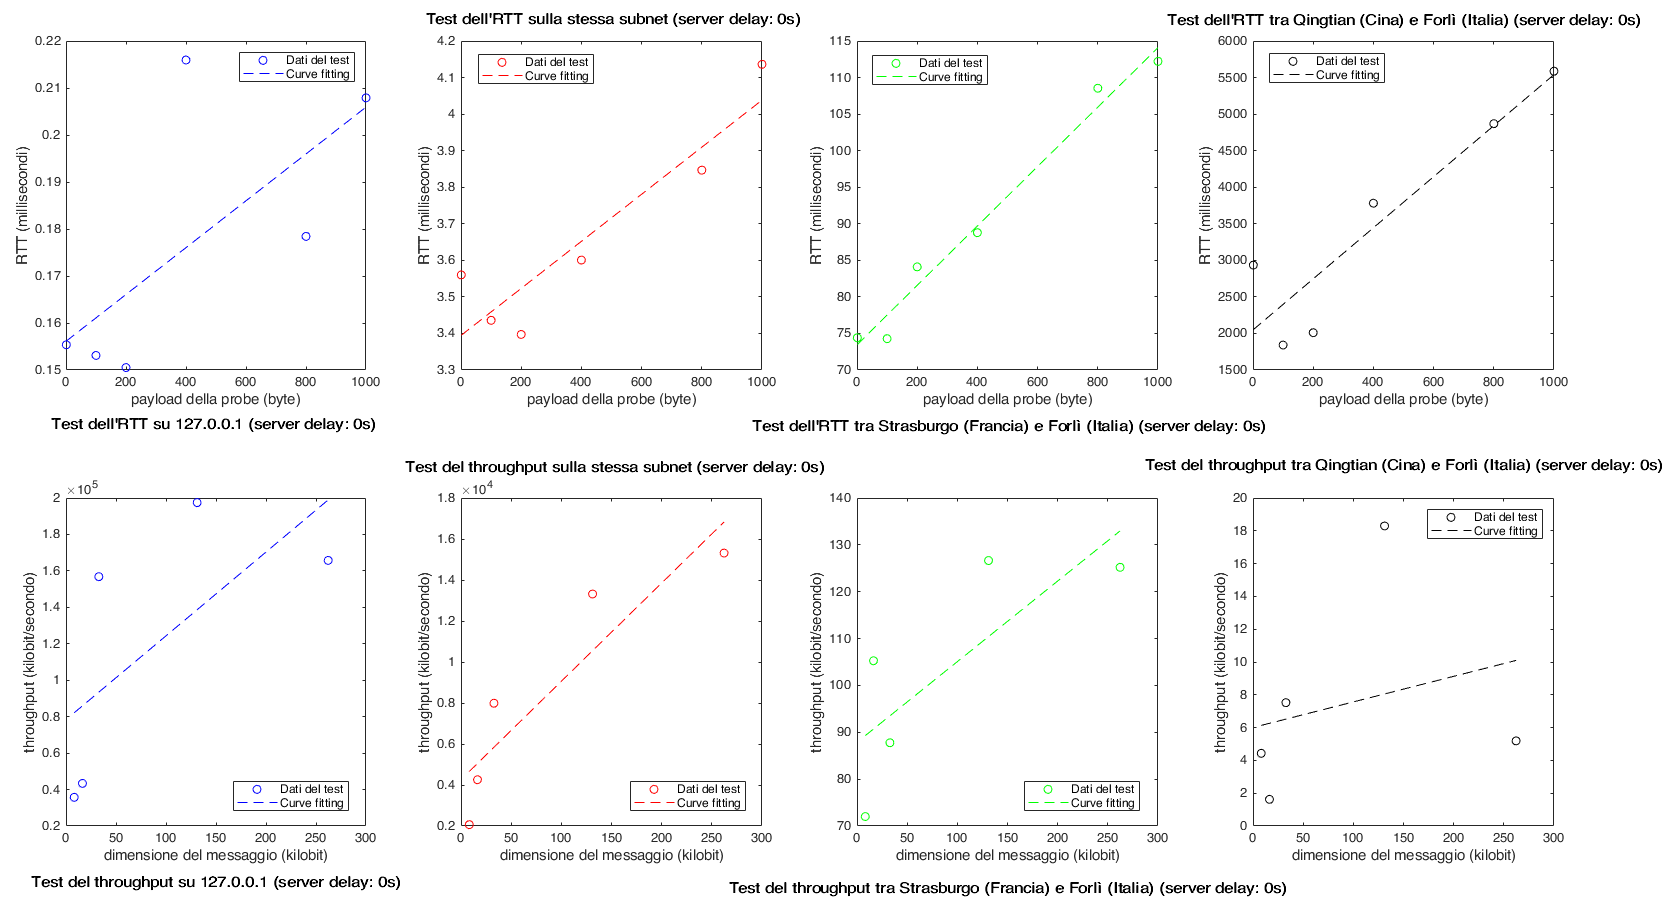
\includegraphics[width=\linewidth]{images/nodelay.png}
	\caption{Grafici con i test effettuati senza ``\textit{server delay}"}
\end{figure}

All'aumentare della distanza tra \textit{client} e \textit{server} tra i vari grafici, l'RTT aumenta il proprio ordine di grandezza, passando
dai decimi di millisecondo ai secondi, segno che aumentando la distanza si aumenta anche il ritardo di propagazione che finisce per aumentare il
valore dell'RTT.\newline
Per il \textit{throughput}, anziché aumentare gli ordini di grandezza muovendosi verso destra tra i grafici, quello che succede è che l'ordine
di grandezza cala. Questo perché i dati inviati mantengono un'insieme di dimensioni costanti tra i test, mentre l'RTT aumenta.\newline
All'aumentare del \textit{payload} della probe l'RTT aumenta, perché è necessario dover immettere sulla rete un numero sempre 
crescente di byte, aumentando il valore del ritardo di trasmissione, che anch'esso va ad aumentare il valore dell'RTT.\newline
Contrariamente alle aspettative, però, all'aumentare delle dimensioni del messaggio, il \textit{throughput} aumenta e non diminuisce. Questo perché
l'aumento dei dati trasmessi è sempre maggiore dell'aumento subito dall'RTT per trasportare più dati.

\begin{figure}[H]
	\centering
	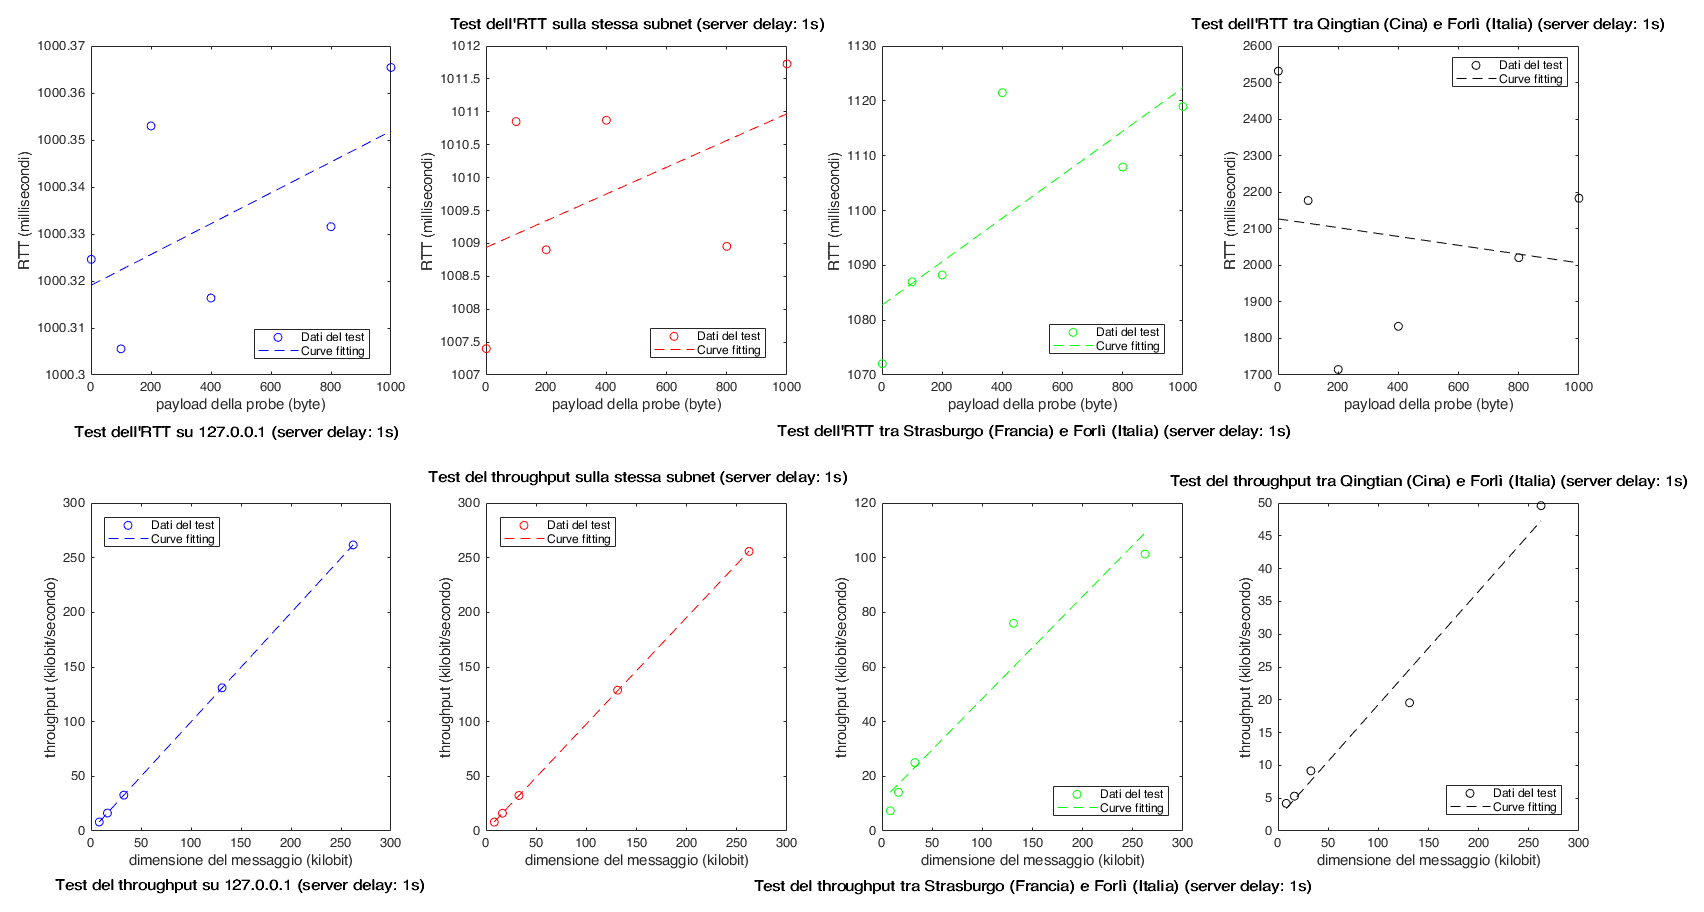
\includegraphics[width=\linewidth]{images/delay.png}
	\caption{Grafici con i test effettuati con ``\textit{server delay}" posto ad un secondo}
\end{figure}

Aggiungendo un ``\textit{server delay}" di un secondo, le osservazioni fatte in precedenza rimangono inalterate. Fa eccezione il quarto grafico della
prima riga dove la linea di tendenza ha pendenza negativa anziché positiva, ma questo è dovuto al primo punto che è molto in alto rispetto
agli altri, mentre gli altri sono pressoché allineati in maniera crescente, permettendo di etichettarlo come un dato trascurabile.\newline
L'uso di un ``\textit{server delay}" così alto rispetto ai valori degli RTT misurati senza \textit{delay} riesce però nell'uniformare l'ordine di grandezza 
del \textit{throughput}.

\end{document}
